\documentclass[12pt, letterpaper]{article}
\usepackage{graphicx}

\title{Pymagicc: A Python wrapper for the simple climate model MAGICC}
\author{Ehsan Rafiei Azad}
\date{June 20, 2021}

\begin{document}

\maketitle

\section{Introduction}
Pymagicc\footnote{https://github.com/openscm/pymagicc} is a Python wrapper around the reduced complexity climate model MAGICC6\footnote{http://magicc.org/}.  
Pymagicc runs on Windows, macOS and Linux and simplifies usage of the model by
utilising DataFrames from the Pandas library (McKinney 2010) as a data structure for
emissions scenarios. To read and write the text-based MAGICC configuration and output
files in the Fortran Namelist format Pymagicc utilizes the f90nml library (Ward 2017). All MAGICC model parameters and emissions scenarios can thus easily be modified through
Pymagicc from Python. MAGICC (Model for the Assessment of Greenhouse Gas Induced Climate Change) is widely used in the assessment of future emissions pathways in climate policy analyses, e.g. in the Fifth Assessment Report of the Intergovernmental Panel on Climate Change (IPCC 2014). Many Integrated Assessment Models (IAMs) utilize MAGICC to model the
physical aspects of climate change. It has also been used to emulate complex atmosphereocean general circulation models (AOGCM) from the Coupled Model Intercomparison
Projects.

In this project, I use one of preloaded RCP (Representative Concentration Pathway) scenario to create 1 plot, and another plot was created using all four (4) scenarios RCP. 
 


\section{Methods}

\subsection{Dataset}
The demo data provided by MAGICC under RCPs scenarios was used for this demonstration. The RCPs offers four strategies for the coming century, each based on various assumptions about population, economic development, energy use and sources, and land use.
Each RCP scenario describes alternative trajectories for carbon dioxide emissions and the resulting atmospheric concentration from 2000 to 2100 and preloaded in Pymagicc.



\section{Pymagicc data visualization}

\subsection{Concentration to emissions hybrid}
This is the default run mode for MAGICC. MAGICC will operate with preset concentrations (or a quantity that scales linearly with radiative forcing for aerosol species) until a specific point in time. At that point, it will transition to an emissions-driven mode. 

\begin{figure}[H]
\centering
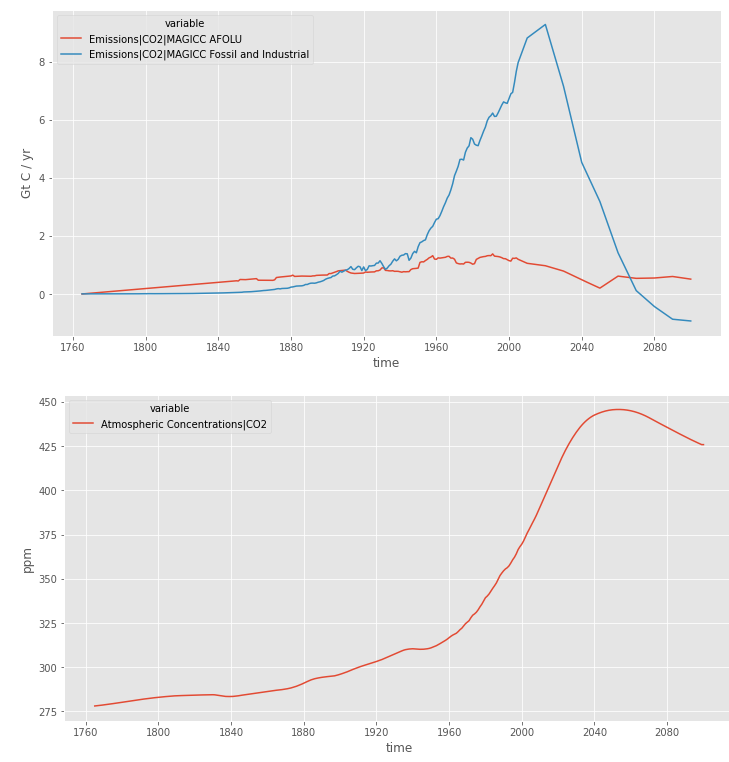
\includegraphics[scale=0.7]{Task1.PNG}
\caption{Concentration to emissions hybrid}
\label{fig:Task1}
\end{figure}

\subsection{Global Mean Temperature Projection}
I created a python script named Task2.py  to visualize the Mean temperature projection from the year of 1850 to 2100.

\begin{figure}[H]
\centering
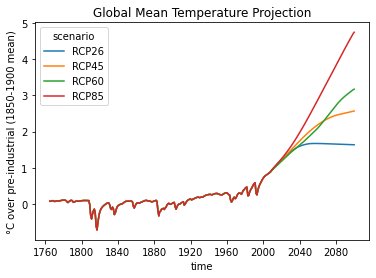
\includegraphics[scale=0.7]{Task2.PNG}
\caption{Global Mean Temperature Projection}
\label{fig:Task2}
\end{figure}

\subsection{Filtering and plotting}
Here it shows how to filter and plot with data, making the most of the capability provided by pyam's IamDataFrame.

\begin{figure}[H]
\centering
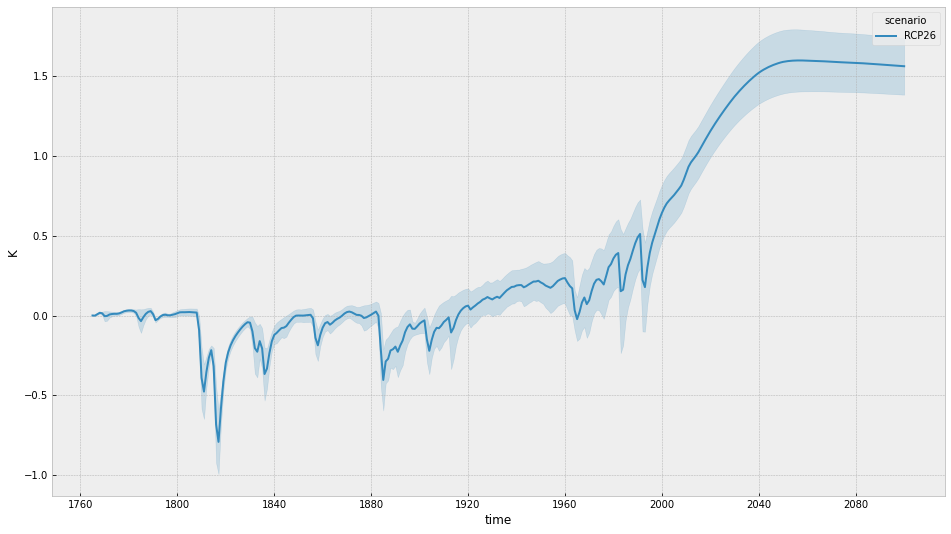
\includegraphics[scale=0.4]{Task3.PNG}
\caption{Filtering and plotting}
\label{fig:Task3}
\end{figure}

\section{Conclusions}
After completion this project, I can conclude that I have tried to learn that how to utilize third party python library or framework such as Pymagicc to develop python software and how to generate useful plots using that framework.

\end{document}